\documentclass[10pt,utf8]{beamer}

\mode<presentation> {
  \usetheme{Madrid}
  \setbeamercovered{transparent}
}

\usepackage{palatino}
\usepackage{graphicx}
\usepackage{array}
\usepackage{color}
\usepackage{subfigure}
\usepackage{colortbl}
\usepackage{amsmath}
\usepackage{hyperref}
\usepackage{listings}
\usepackage{pythonhighlight} % dnf install texlive-pythonhighlight

\setbeamertemplate{caption}{\raggedright\insertcaption\par} %turn off caption prefix ("Figure")


\title{Feeding ML models with the data from the databases in real-time}
\author{Vojtěch Juránek}
\institute[Red Hat]{Red Hat}
\date{Feb. 3rd 2024, FOSDEM, Brussels}

\newenvironment{mylisting}
{\begin{list}{}{\setlength{\leftmargin}{1em}}\item\scriptsize\bfseries}
{\end{list}}

\newenvironment{mytinylisting}
{\begin{list}{}{\setlength{\leftmargin}{1em}}\item\tiny\bfseries}
{\end{list}}


\begin{document}

%\tikzstyle{every picture}+=[remember picture]
%\tikzstyle{na} = [baseline=-.5ex]


\begin{frame}
 \titlepage
\end{frame}


\begin{frame}
    \begin{figure}
        \centering
        \includegraphics[height=8cm]{./img/mlops.eps}
        \caption{\tiny{Source: \url{https://ml-ops.org/content/end-to-end-ml-workflow}}}
    \end{figure}
\end{frame}

\begin{frame}
    \begin{figure}
        \centering
        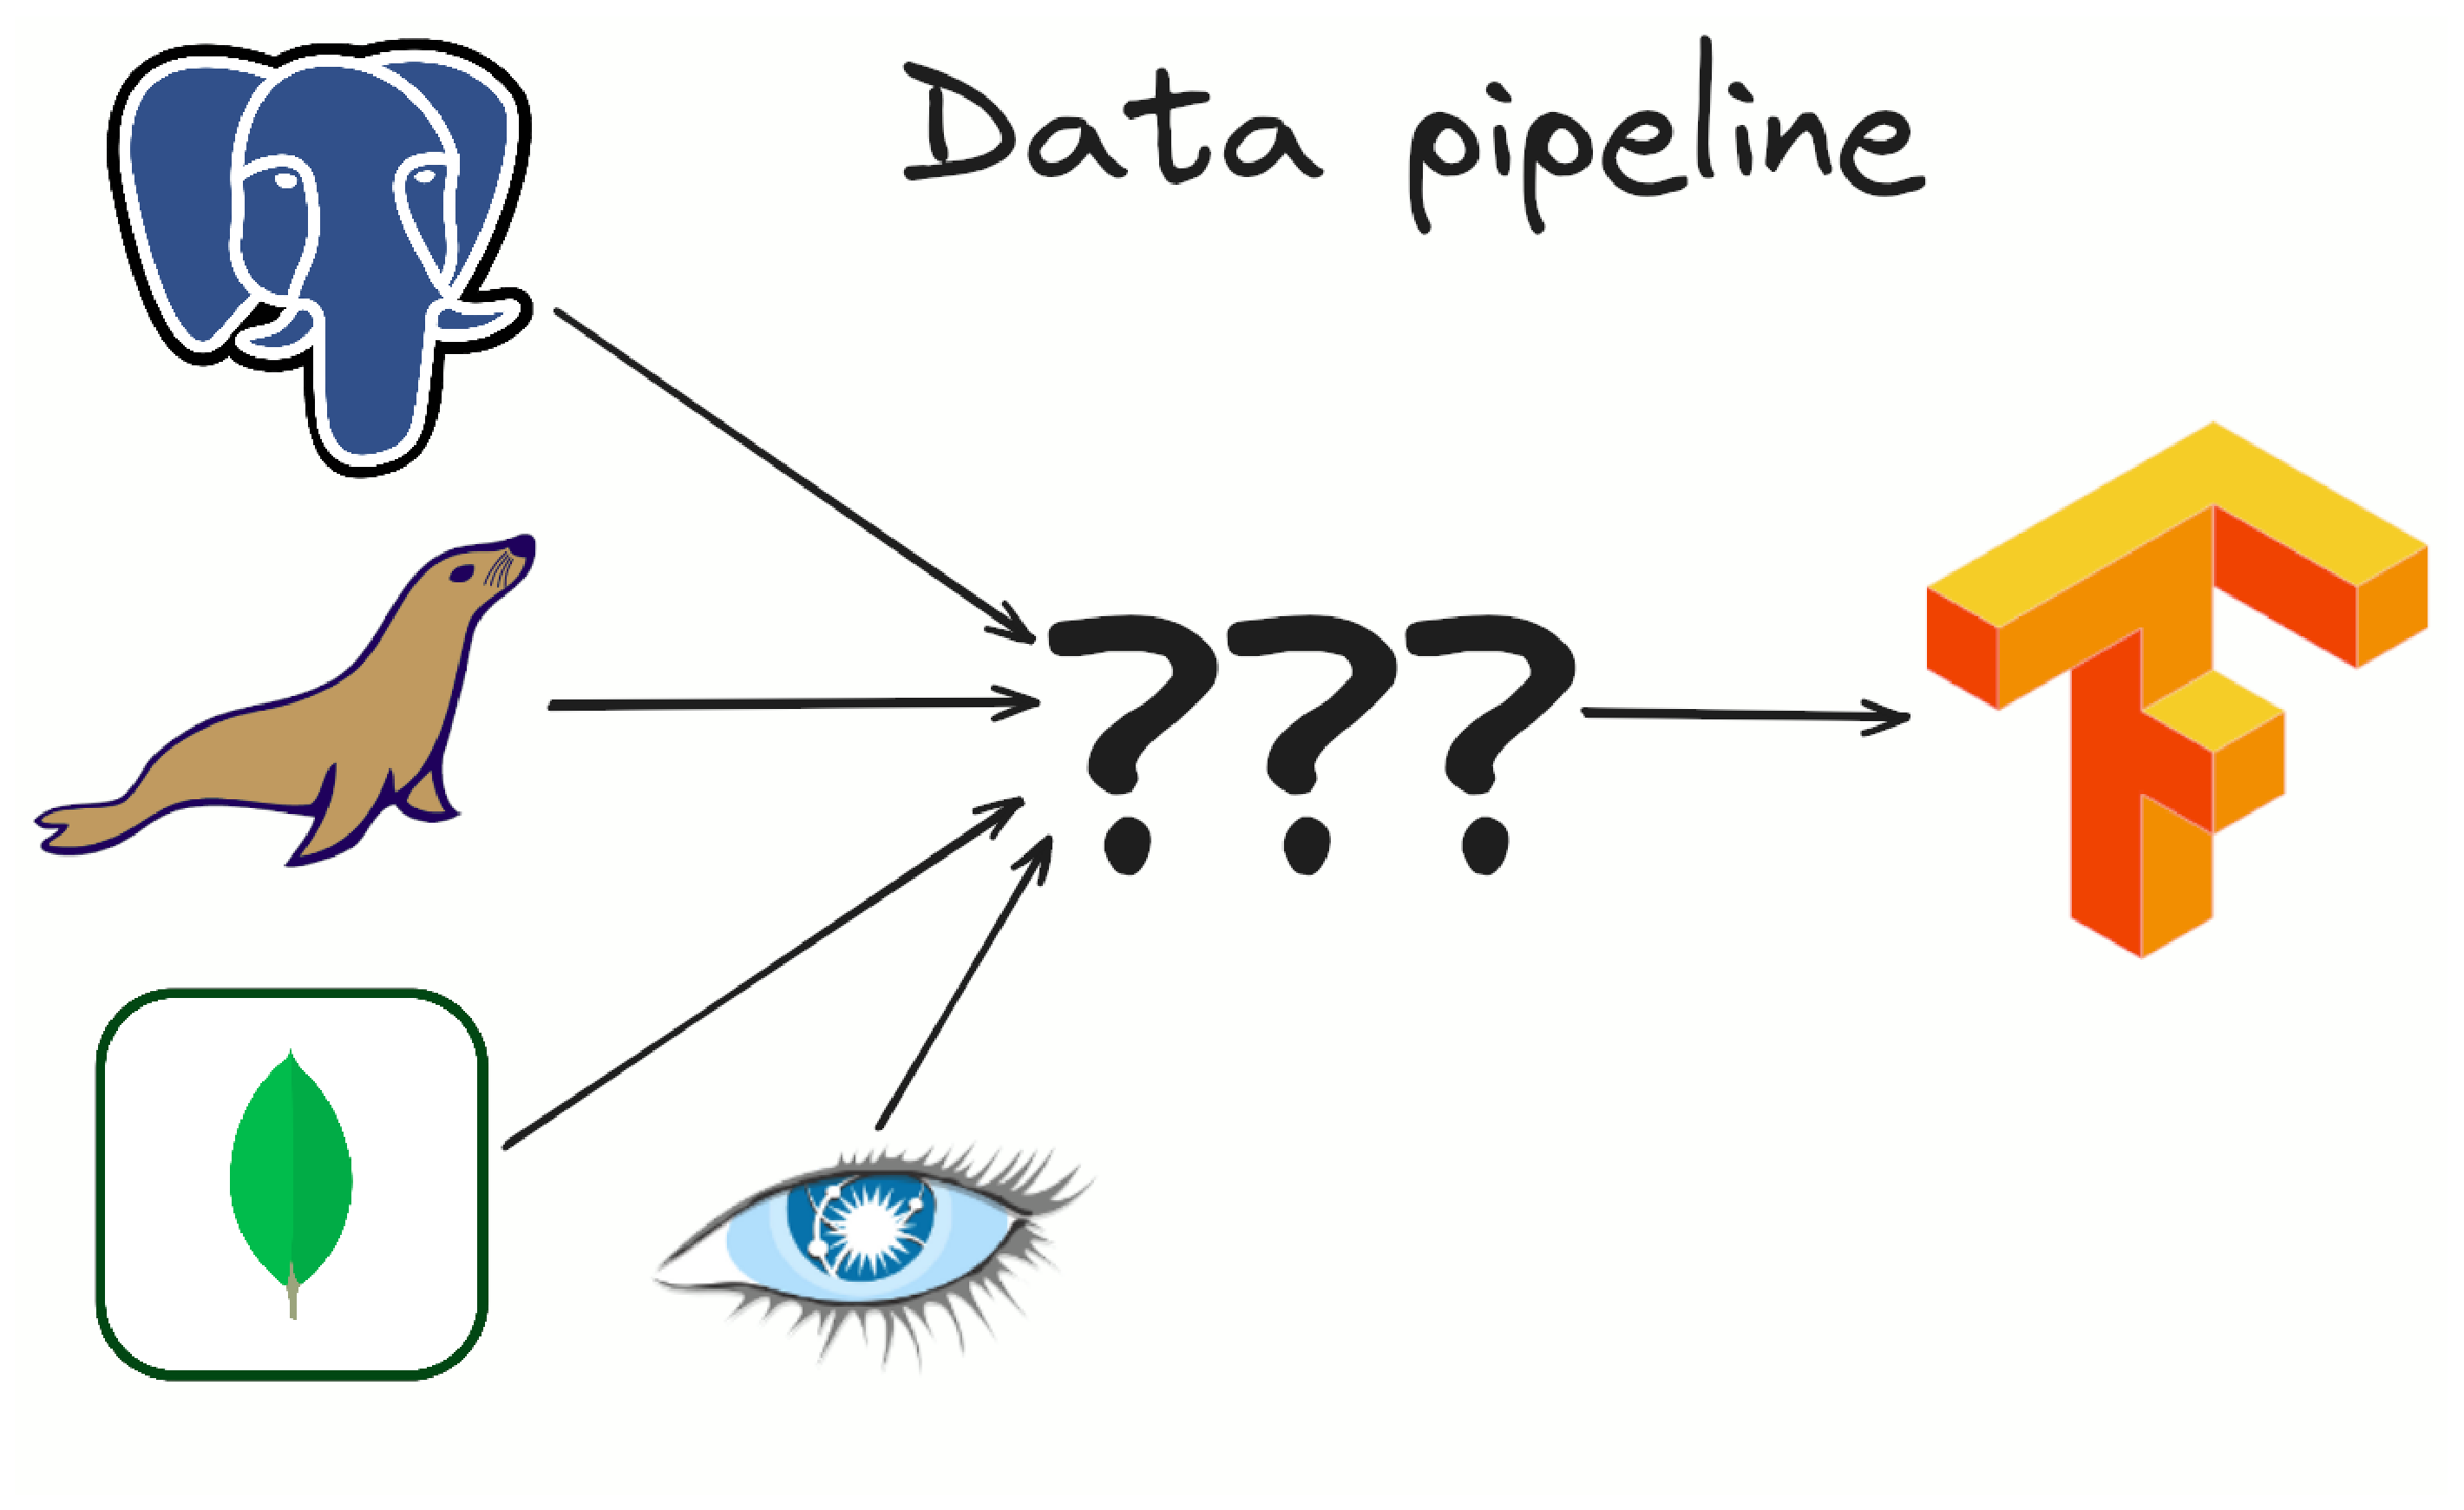
\includegraphics[height=6cm]{./img/dbs_to_tf2.eps}
    \end{figure}
    \begin{itemize}
      \item Consistent data, no data losses, no dual writes.
      \item Get all the changes without any delay in the real-time.
      \item Not overload the DB with the queries.
    \end{itemize}
\end{frame}

\begin{frame}
   % \frametitle{Change Data Capture (CDC)}
    \begin{figure}
        \centering
        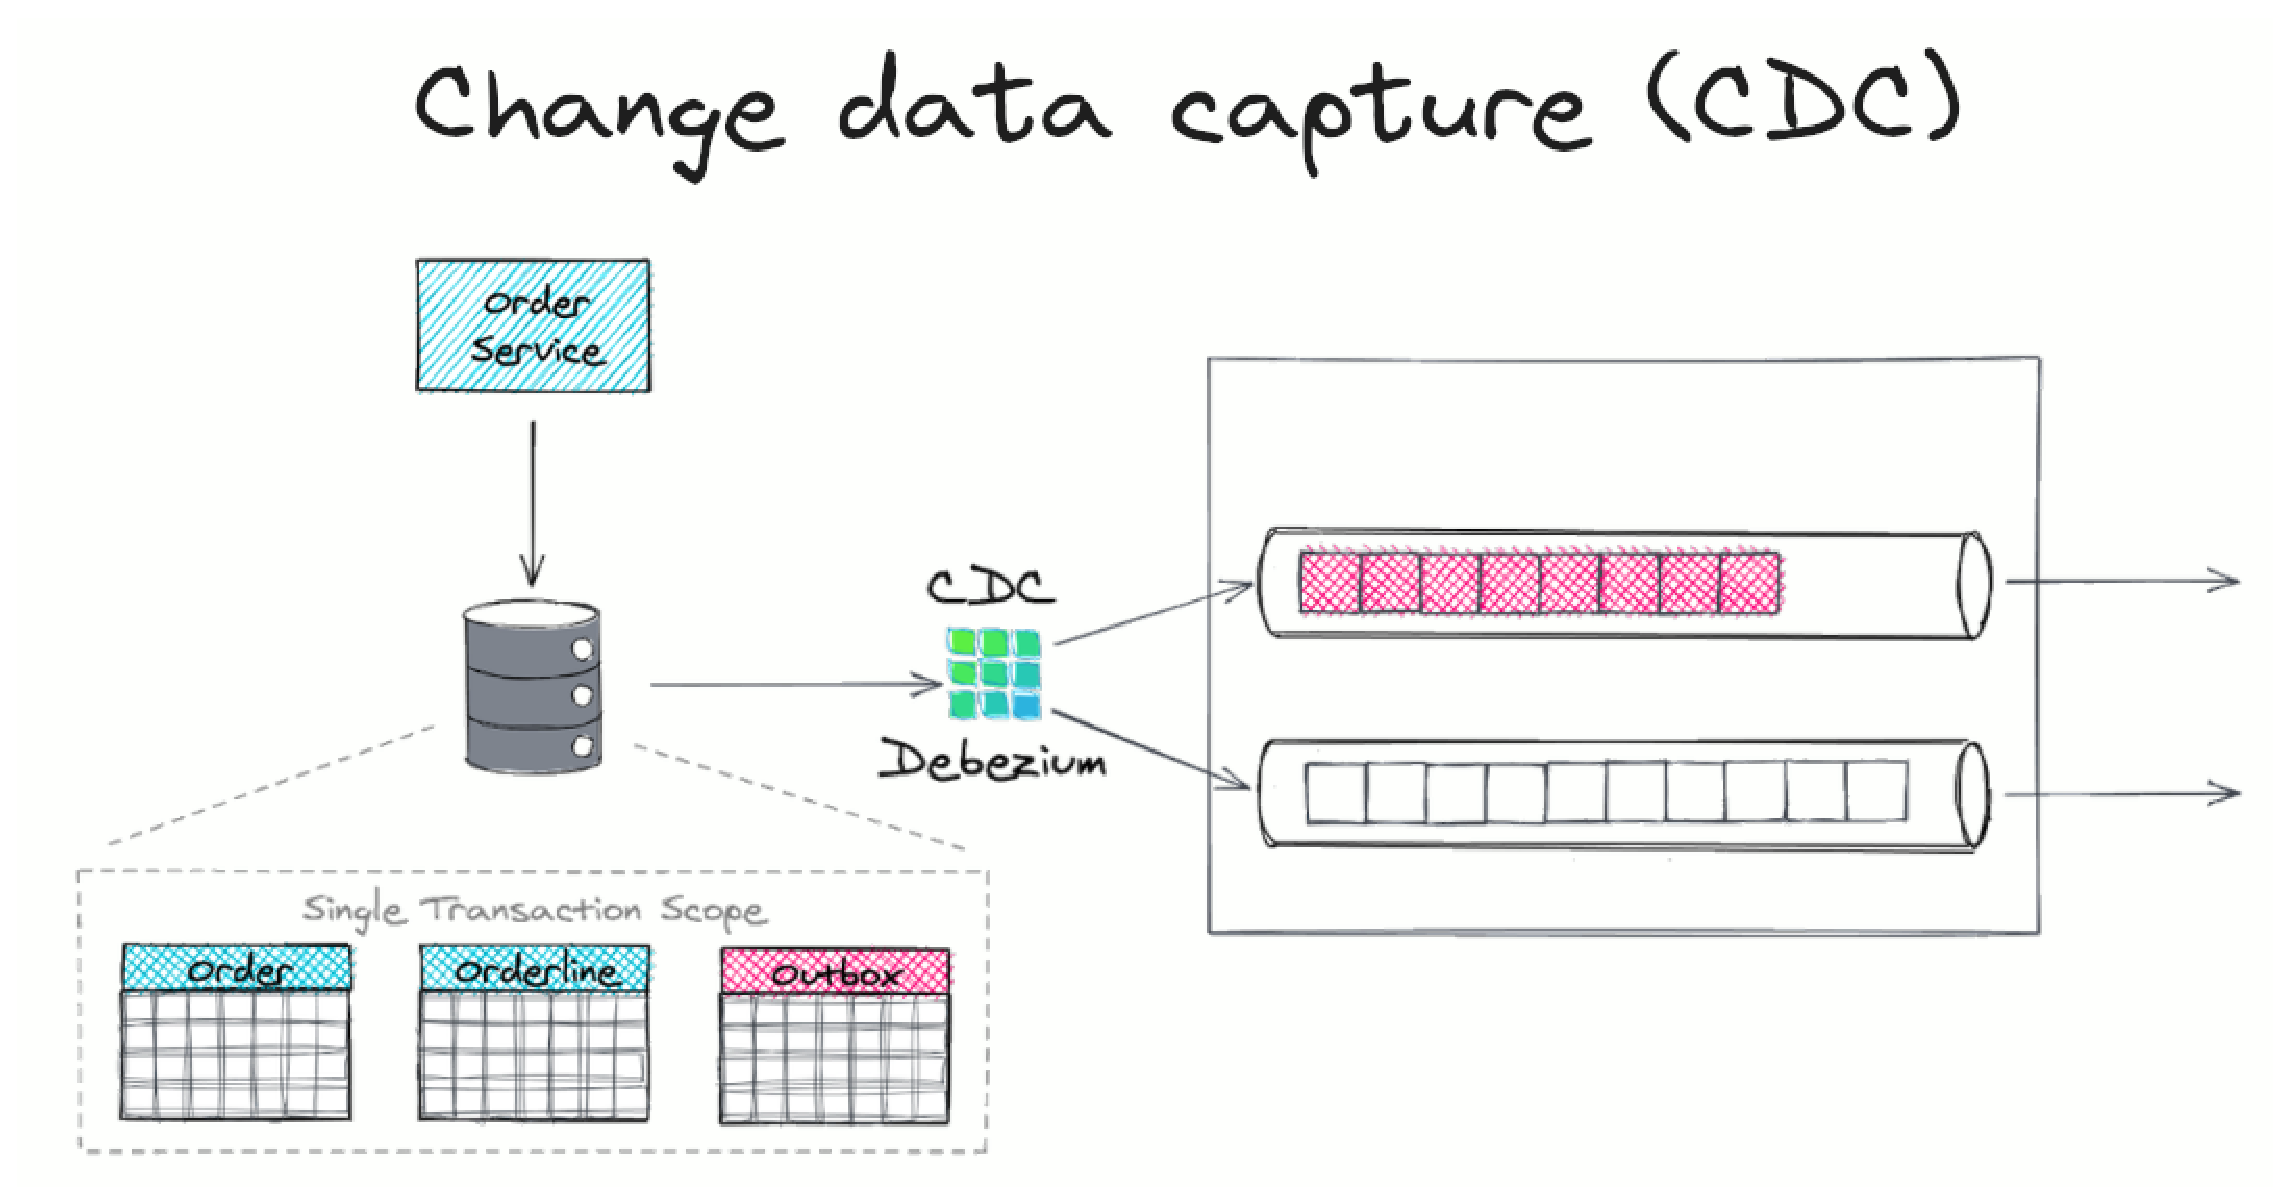
\includegraphics[height=6.5cm]{./img/cdc2.eps}
    \end{figure}
\end{frame}

\begin{frame}
    \begin{figure}
        \centering
        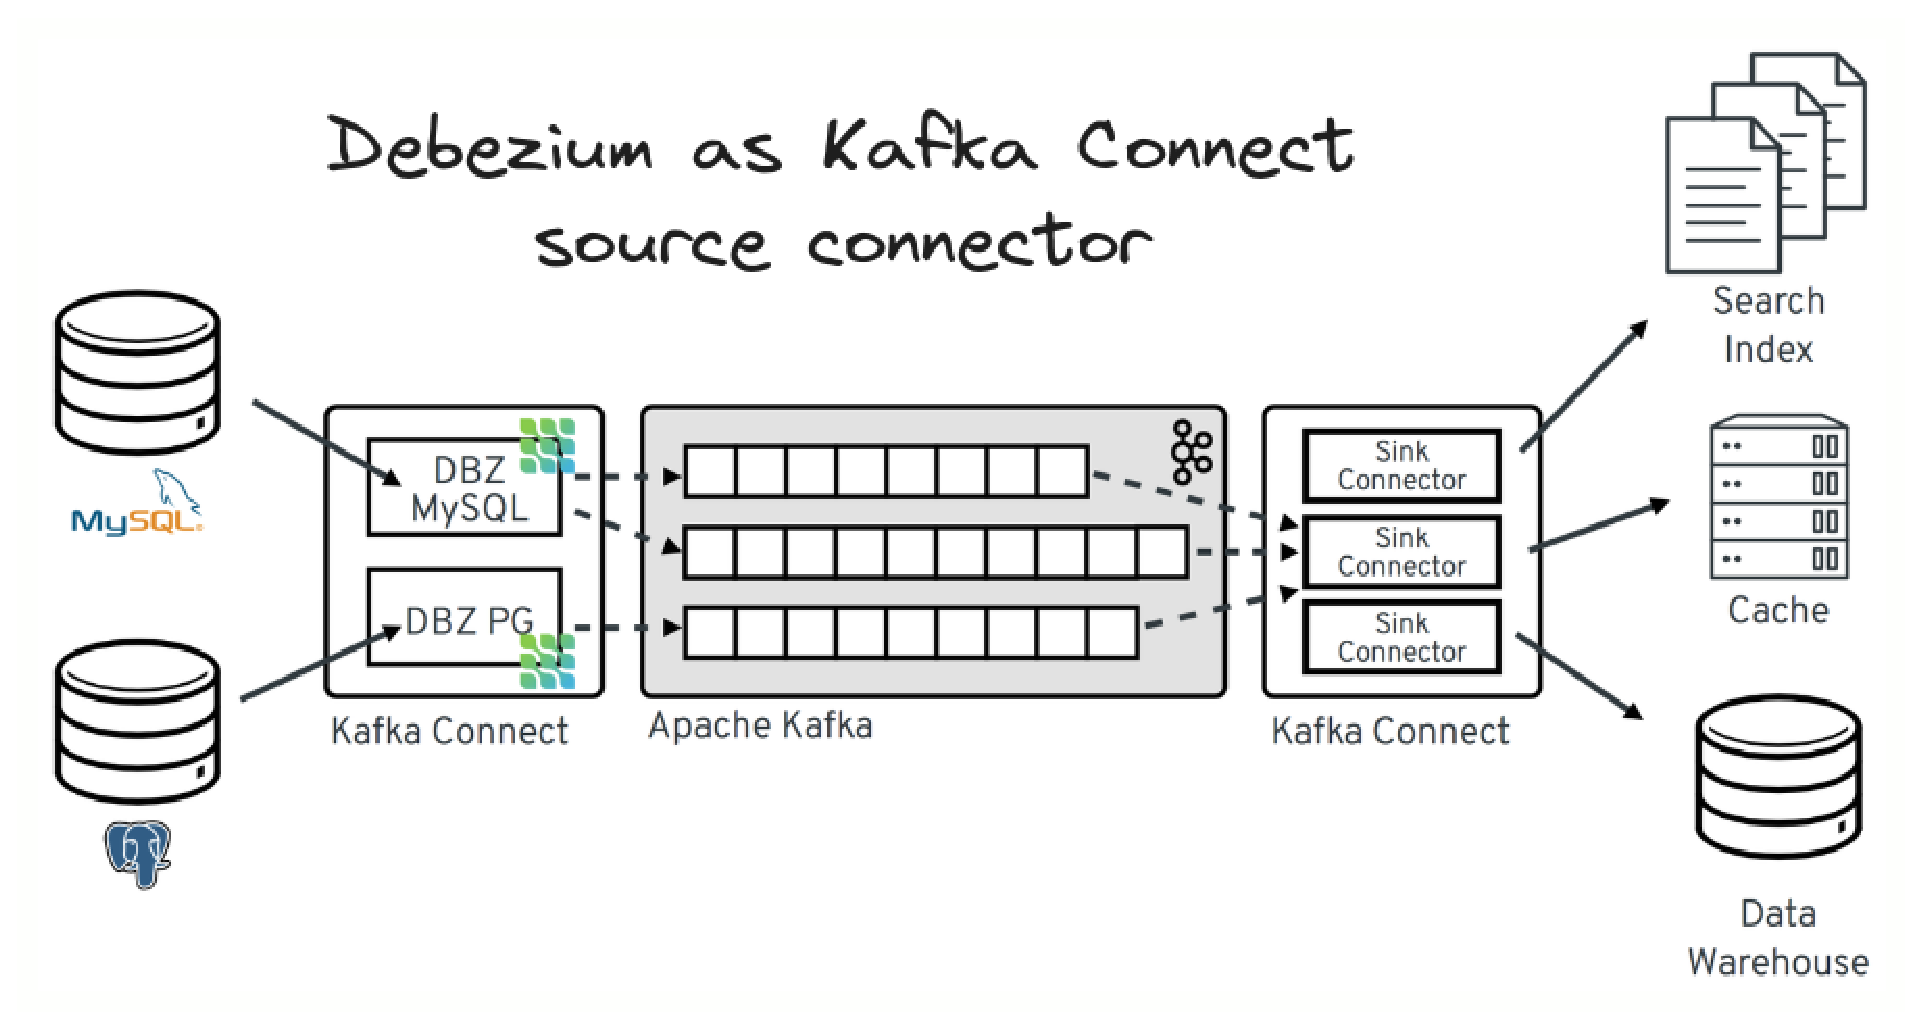
\includegraphics[height=5cm]{./img/debezium_kafka.eps}
    \end{figure}
    
    \vspace{-0.5cm}
    
    \begin{figure}
        \centering
        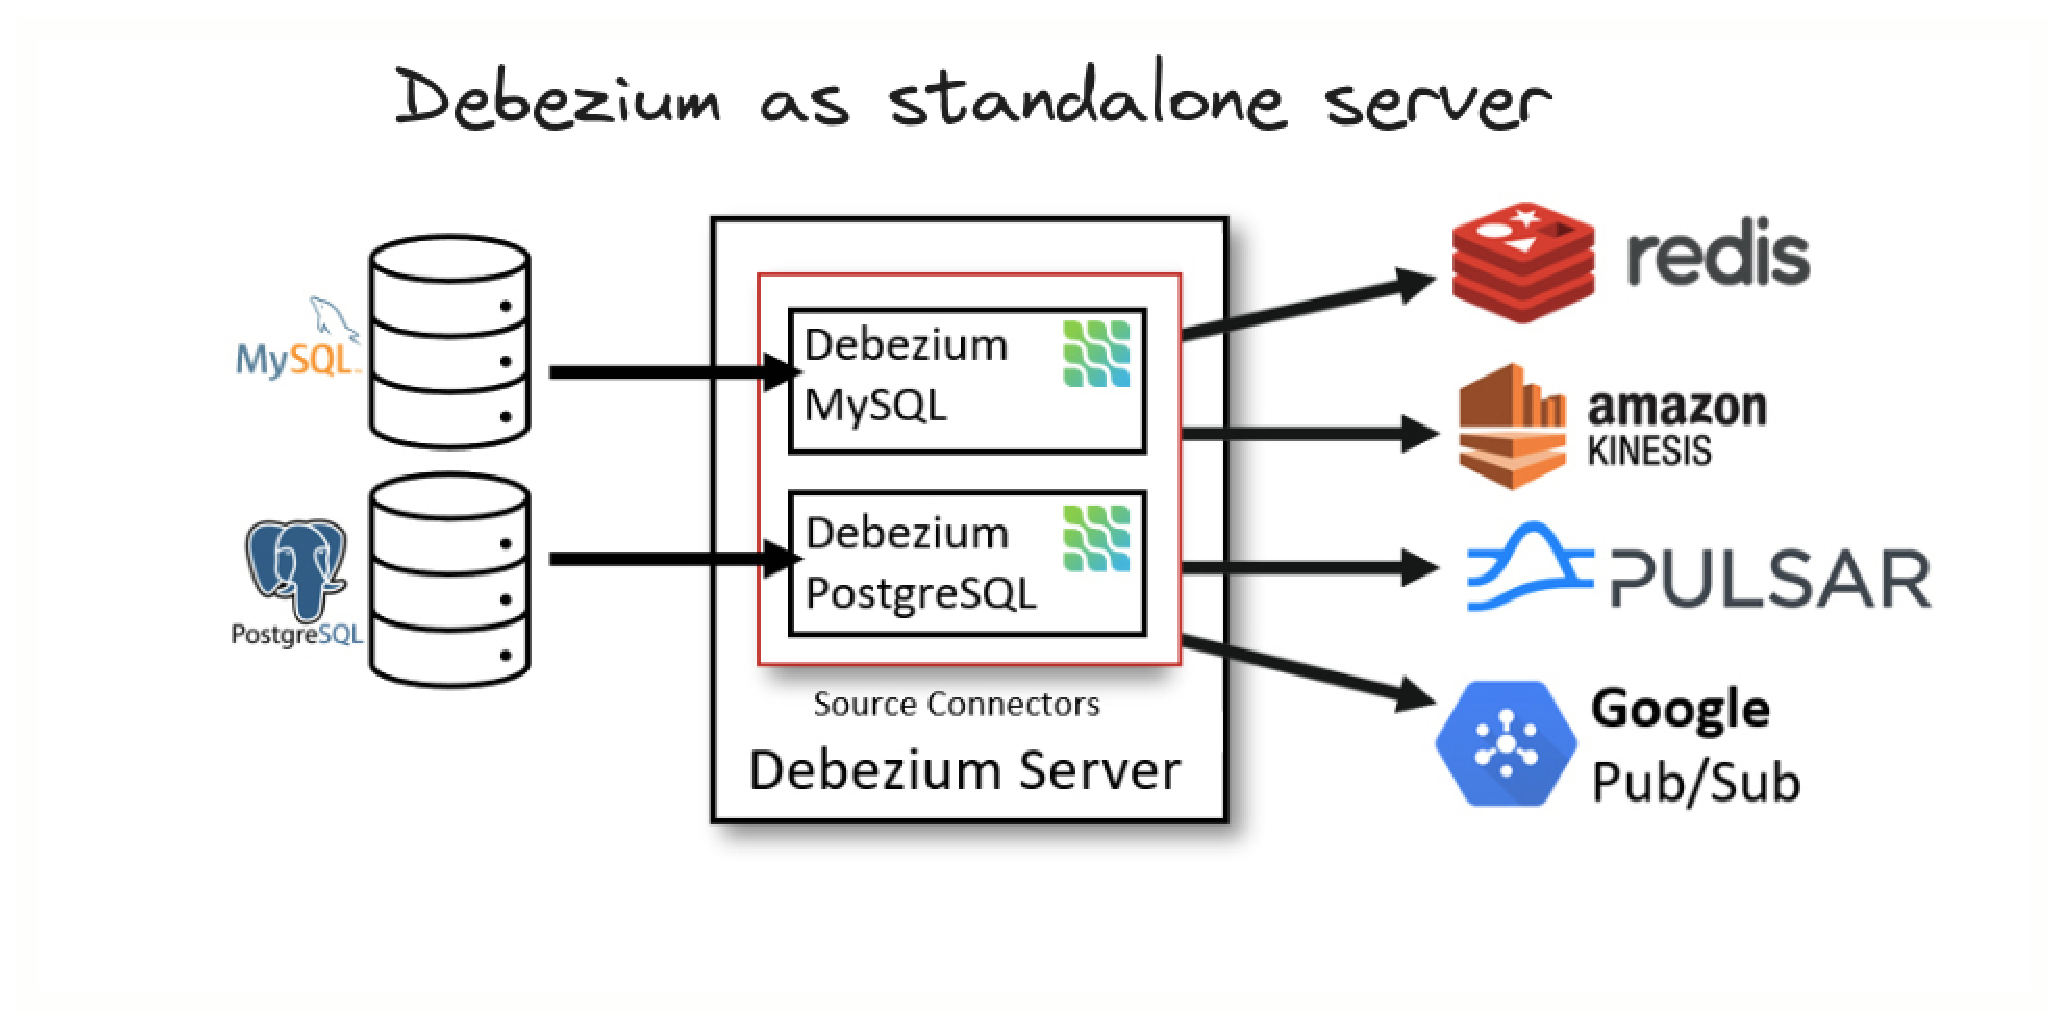
\includegraphics[height=5cm]{./img/debezium_server.eps}
    \end{figure}
\end{frame}

\begin{frame}
    \frametitle{Debezium}
    \vspace*{-3cm}
    \begin{figure}
        \hspace*{-1.4cm}
        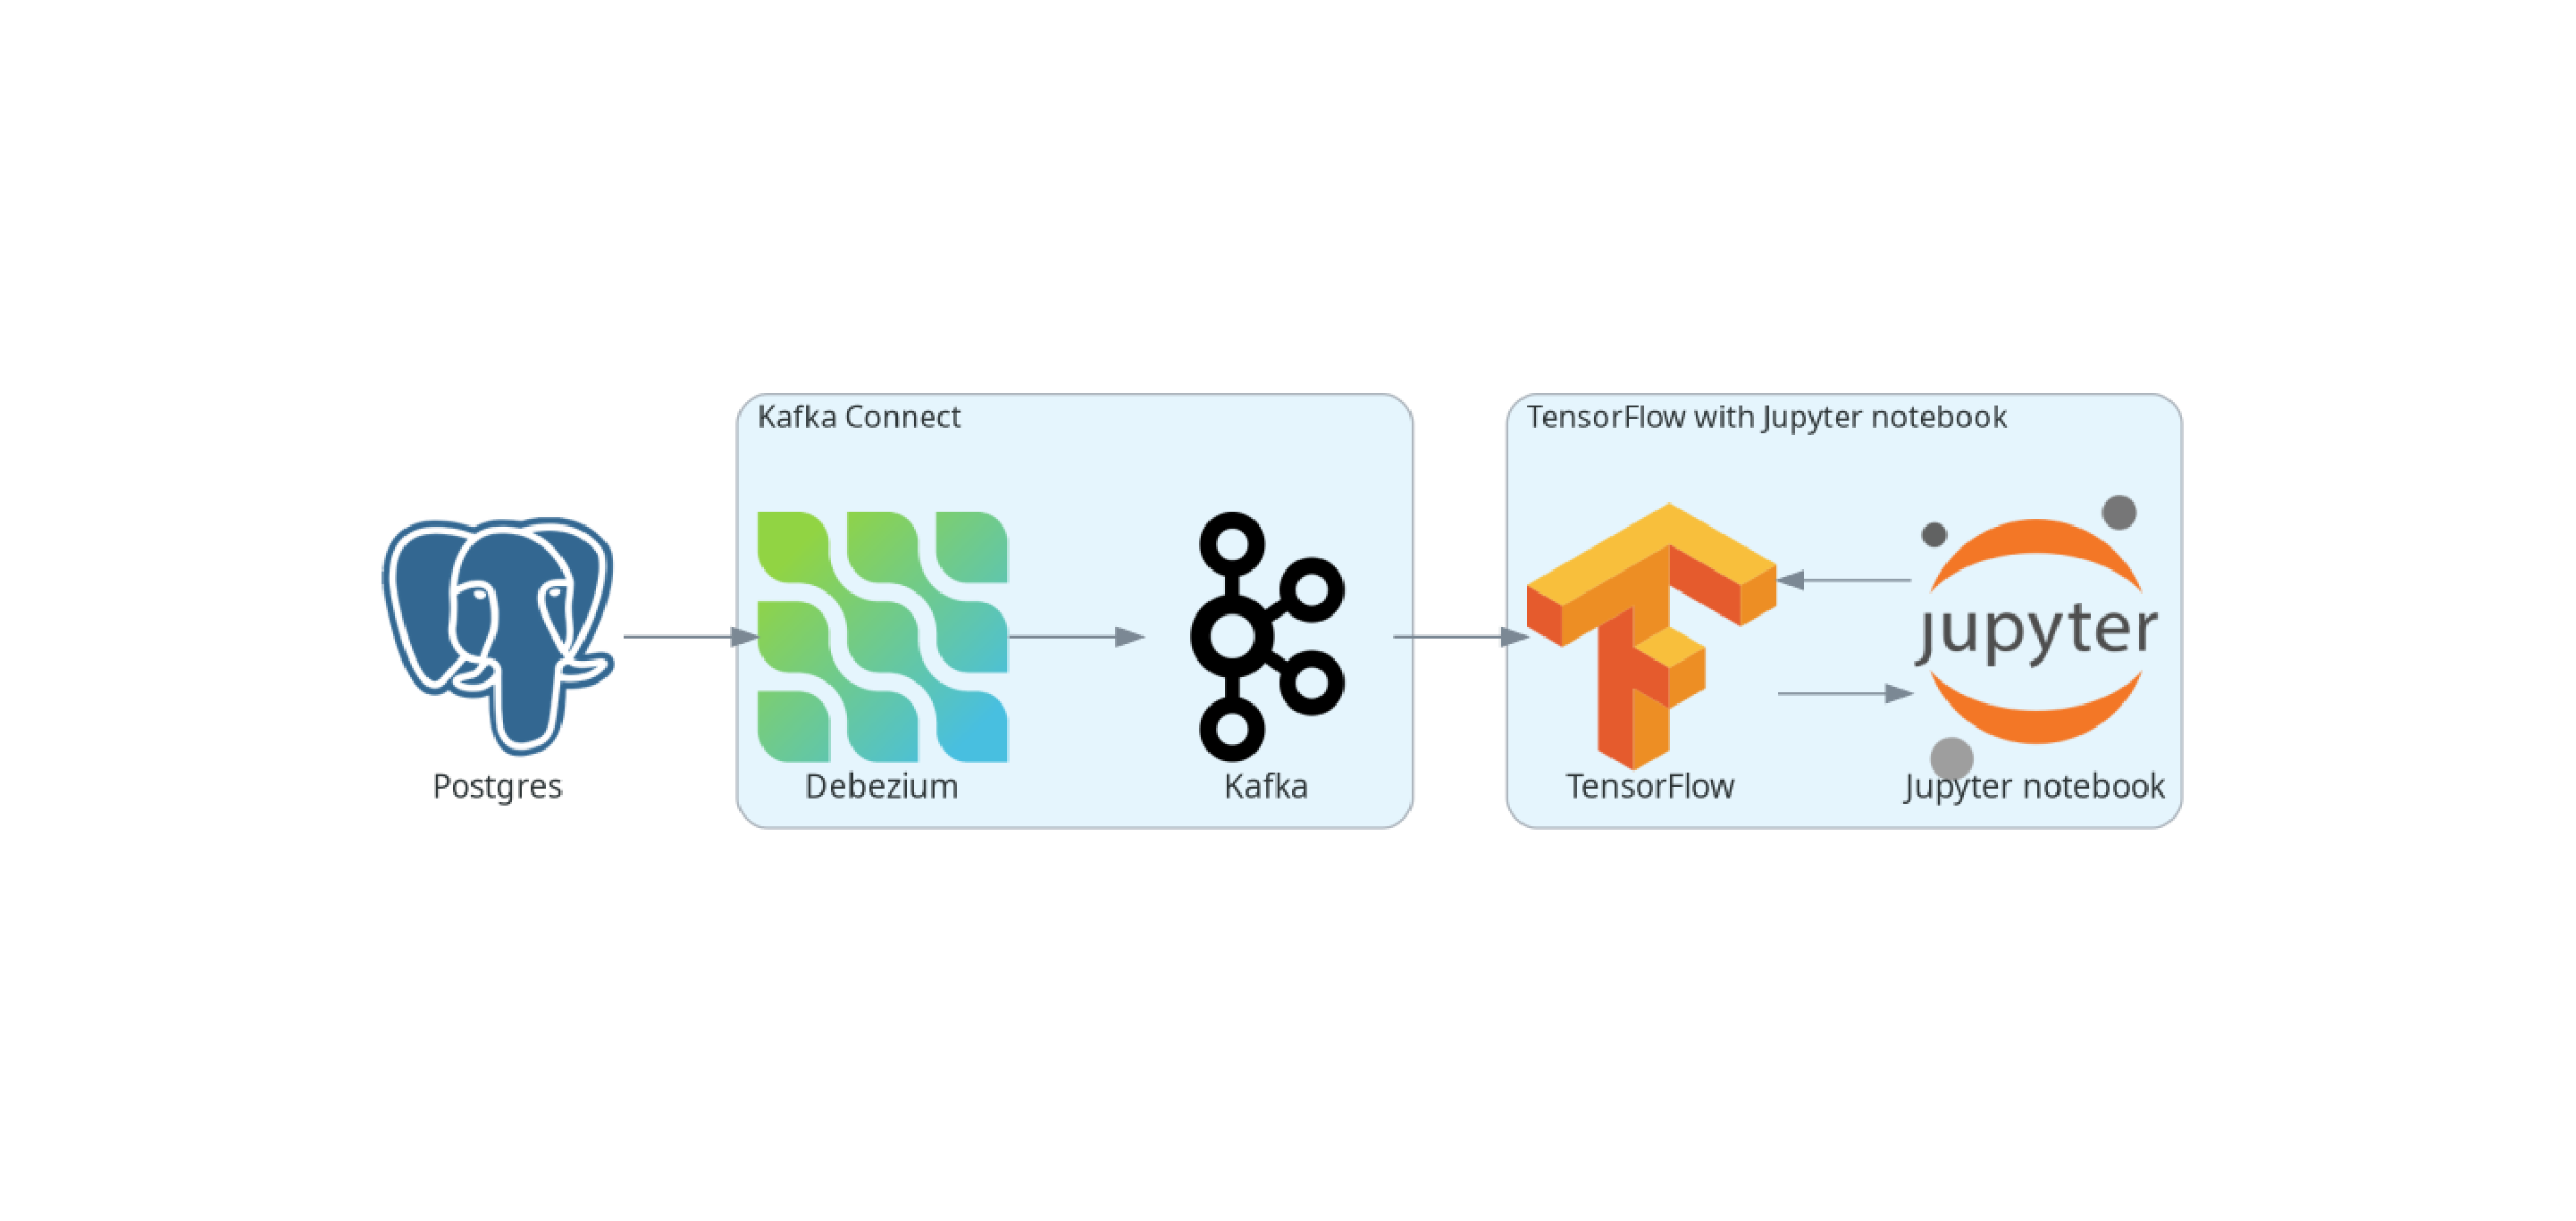
\includegraphics[height=7cm]{./img/postgres_to_tf.eps}
    \end{figure}
    
    For more details see
    \begin{itemize}
        \item  \footnotesize \color{blue}\url{https://debezium.io/blog/2023/05/02/tensorflow-mnist-classification}\color{black}
        \item  \footnotesize \color{blue}\url{https://github.com/debezium/debezium-examples/tree/main/machine-learning/tensorflow-mnist}\color{black}
    \end{itemize}
\end{frame}

\begin{frame}[fragile]
    \footnotesize
    %\begin{lstlisting}
    \begin{python}
# define function for decoding Kafka records
def decode_kafka_stream_record(message, key):
    img_int = tf.io.decode_csv(message, [[0.0] for i in range(NUM_COLUMNS)])
    img_norm = tf.cast(img_int, tf.float32) / 255.
    label_int = tf.strings.to_number(key, out_type=tf.dtypes.int32)
    return (img_norm, label_int)

# define Kafka data stream
test_ds = tfio.experimental.streaming.KafkaGroupIODataset(
    topics=[KAFKA_TEST_TOPIC],
    group_id=KAFKA_CONSUMER_GROUP,
    servers=KAFKA_SERVERS,
    stream_timeout=KAFKA_STREAM_TIMEOUT,
    configuration=[
        "session.timeout.ms=10000",
        "max.poll.interval.ms=10000",
        "auto.offset.reset=earliest"
    ],
)

# read batches of Kafka records
test_ds = test_ds.map(decode_kafka_stream_record)
test_ds = test_ds.batch(BATCH_SIZE)

# make predictions on the data samples
model.evaluate(test_ds)
    \end{python}
    %\end{lstlisting}
\end{frame}


\begin{frame}
    \begin{figure}
        \centering
        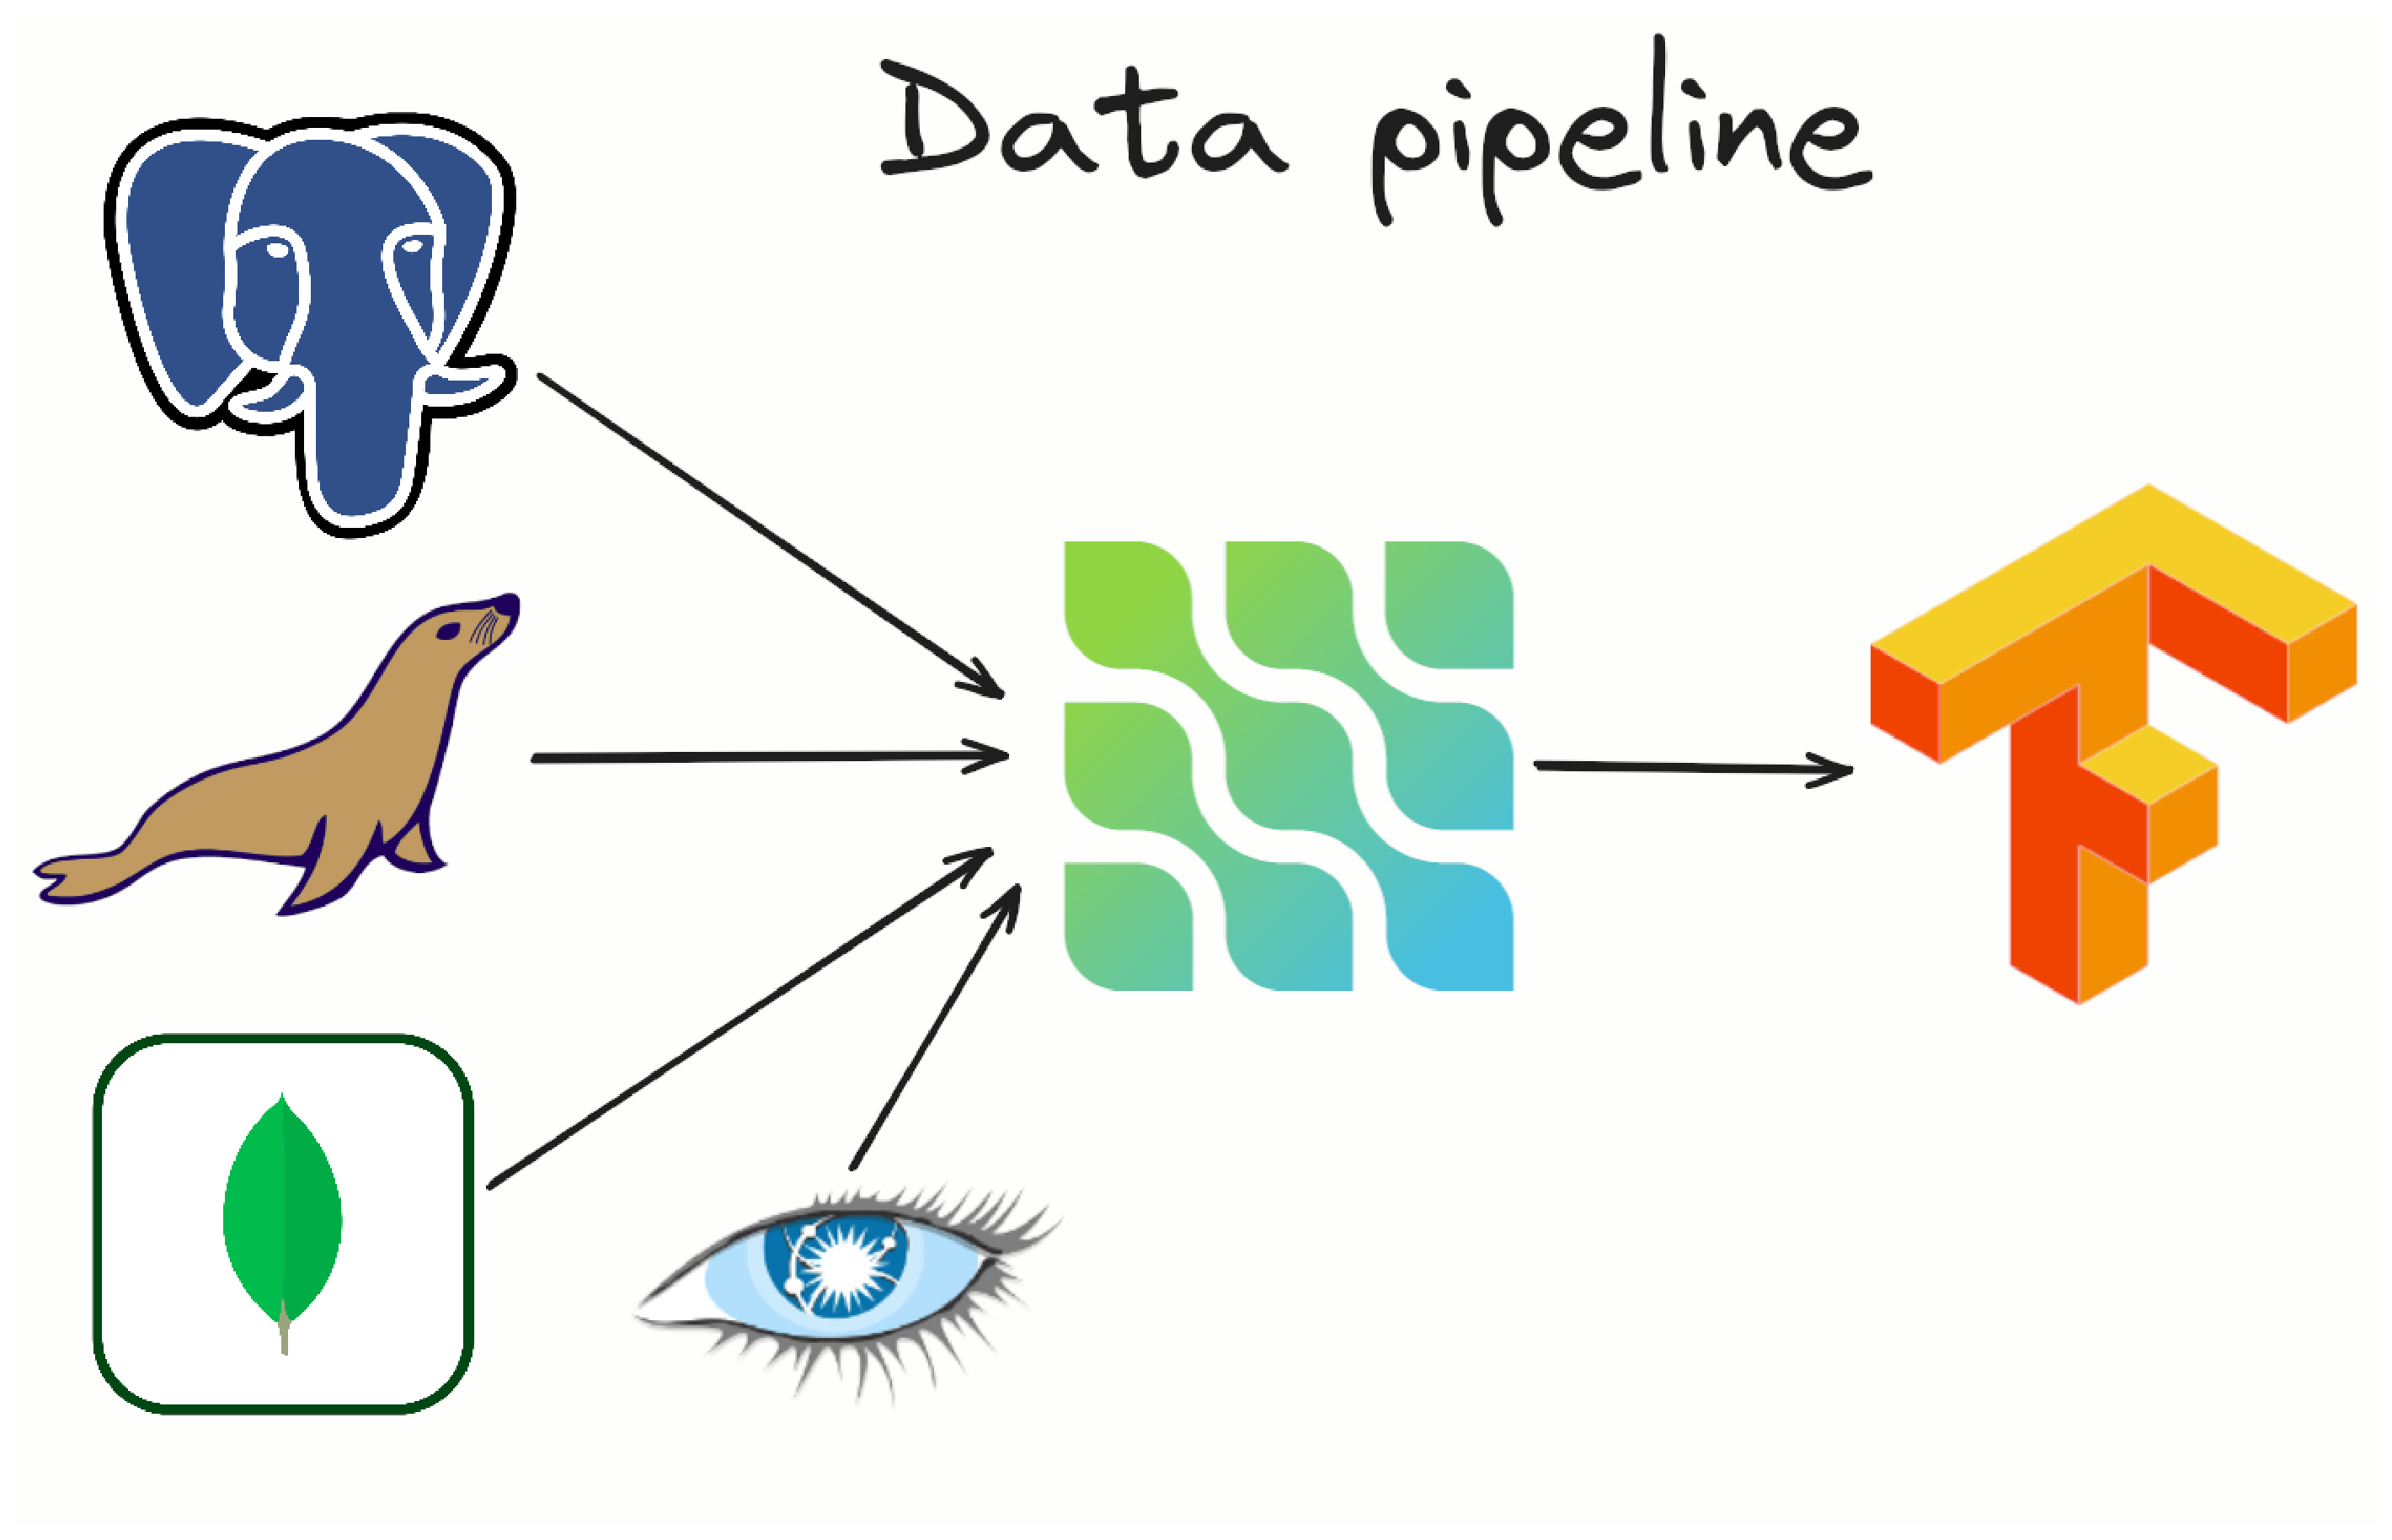
\includegraphics[height=6cm]{./img/dbs_to_tf_debezium.eps}
    \end{figure}
\end{frame}

\begin{frame}
    \centering
    \textbf{\Huge{Thank you!}}
    
    \vspace{1cm}
    
    \begin{figure}
        \centering
        
\includegraphics[height=1.5cm]{./img/debezium.eps}
    \end{figure}
    
    \vspace{0.5cm}
    
    \centering
    \color{blue}\url{https://debezium.io}\color{black} \\
    \color{blue}\url{https://debezium.zulipchat.com}\color{black} \\
    \color{blue}\url{https://github.com/debezium}\color{black} \\
\end{frame}

%%%%%%%%%%%%%%%%%%%%%%%%%%%%%%%%%%%%%%%%%%%%%%%%%%%%%%%%%%%%%%%%%%%%%%%%%%%%%%%%%%%%%%%%%%%%%%%%%
%%% BACKUP
%%%%%%%%%%%%%%%%%%%%%%%%%%%%%%%%%%%%%%%%%%%%%%%%%%%%%%%%%%%%%%%%%%%%%%%%%%%%%%%%%%%%%%%%%%%%%%%%%

\begin{frame}
	\centering
	\huge{\textbf{Backup slides}}
\end{frame}

\begin{frame}
    \begin{figure}
        \hspace*{-1.1cm}
        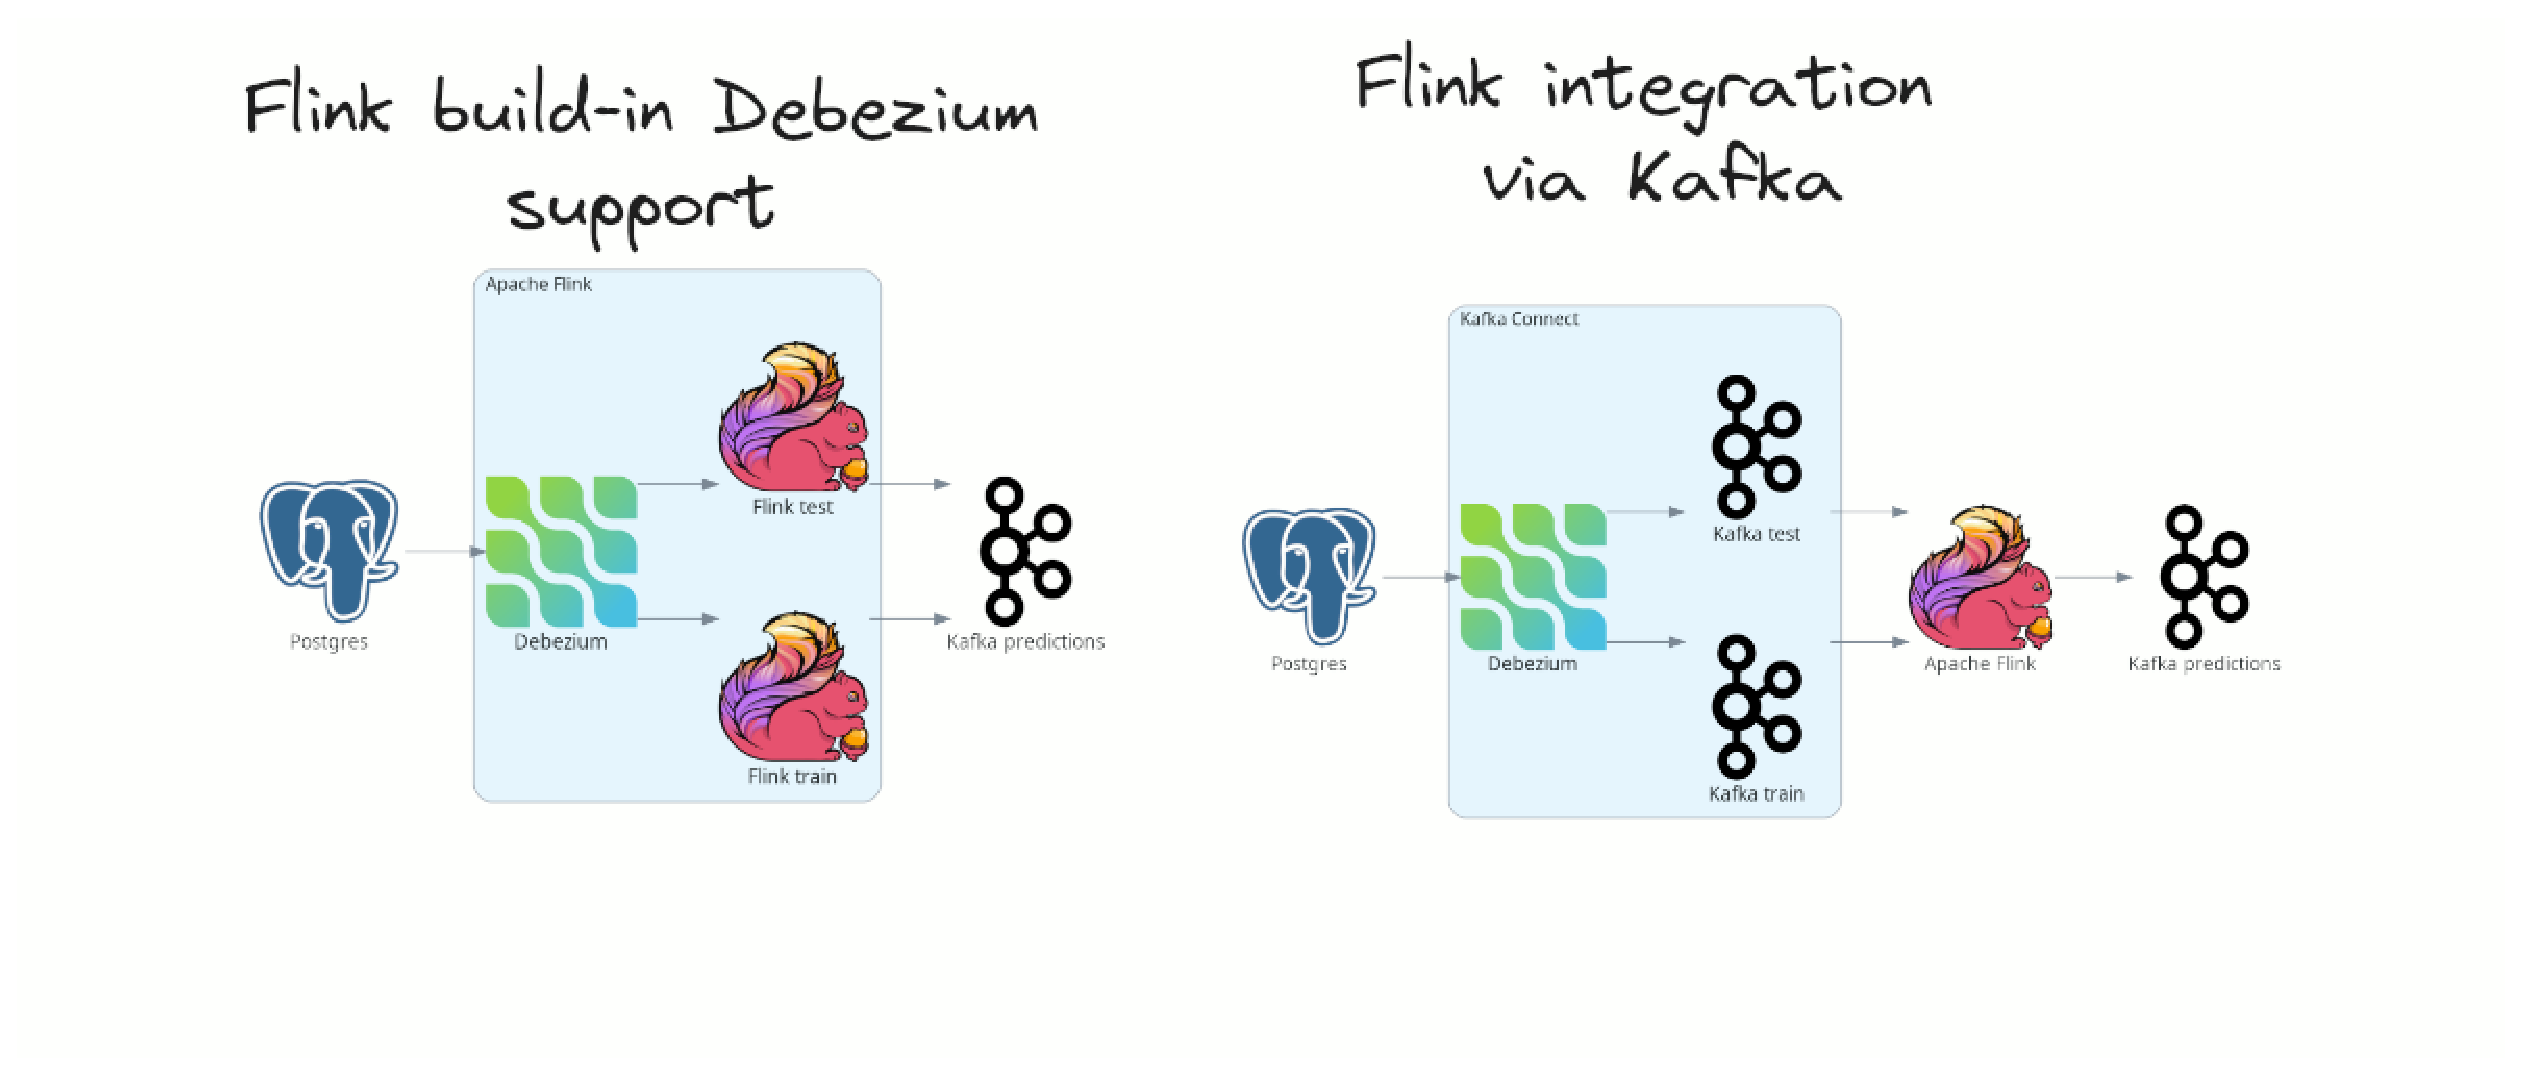
\includegraphics[height=6cm]{./img/debezium_flink.eps}
    \end{figure}
    
    \vspace{-1cm}
    Similar for Apache Spark.
    \vspace{0.5cm}
    
    For more details see
    \begin{itemize}
        \item  \footnotesize \color{blue}\url{https://debezium.io/blog/2023/09/23/flink-spark-online-learning}\color{black}
        \item  \footnotesize \color{blue}\url{https://github.com/debezium/debezium-examples/tree/main/machine-learning/flink-spark-iris}\color{black}
    \end{itemize}
\end{frame}

\end{document}
